In this section we evaluate the performance of the \egrine\ model as a function
of several important parameters. We focus in particular on how the
performance of the model changes as a function of the number of runs
included. From these evaluations, we conclude that (1) the model
performs well in its final form, (2) the model has reached a stable-state 
wherein inclusion of additional runs does not significantly increase model
performance, and (3) the model is not over-fit to particular
experiments within a data set or to any data set as a whole.

\subsection{Comparison with other module detection algorithms}

We compared the number of \rdb~TFs detected in the \egrine~model to individual
\cm~runs as well as to several other module detection/clustering
algorithms that were computed on subsets of the experimental data
(similar to the \egrine~ensemble; Figure \ref{fig:ensemble_comparison_regDB}). We
evaluated: (a) $k$-means clustering, (b) \tmsamp{WGCNA}
\cite{Langfelder2008}, and (c) \tmsamp{DISTILLER}
\cite{Lemmens2009}. For (a) and (b), we computed modules 100 times on
random subsets of the {\it E. coli} expression data set (using 200-250
randomly chosen experiments per run; selection criteria were identical
to {\it E. coli} \egrine; see Table~\ref{tab:cmparams:eco}). We then
predicted {\it de novo cis}-regulatory GREs in the promoter regions of genes
in each module using \tmsamp{MEME} (\tmsamp{MEME} parameters were also
identical to \egrine; Table~\ref{tab:cmparams:eco}). For (c), we
performed the comparison using the original modules generated by
\cite{Lemmens2009}. Rather than alter module composition by
re-detection, we instead varied \tmsamp{MEME} parameters applied to
the modules 100 times (again, within the same ranges as those used for
\egrine). TF-GRE matches were assigned by comparing GREs to
\rdb~TF binding sites, as previously described
(Section~\ref{section:tfbs:vs:regdb}).

We found that individual \cm~runs discovered a greater number of
\rdb~binding sites, on average, than the other methods (an average of
41 for \cm, compared to averages of 30, 25, and 29 for $k$-means,
\tmsamp{WGCNA}, and \tmsamp{DISTILLER}, respectively), which is
consistent with previous findings \cite{Reiss2006n}
(Figure~\ref{fig:ensemble_comparison_regDB}). Integration of all
\cm~biclusters into the complete \egrine~ensemble outperformed all
individual \cm~runs (53 total, as described in the Manuscript). This
result is typical of ensemble-based inference approaches, and supports
the value of ensemble integration as part of the \egrine\ model.

\begin{figure}[h!]
\centering
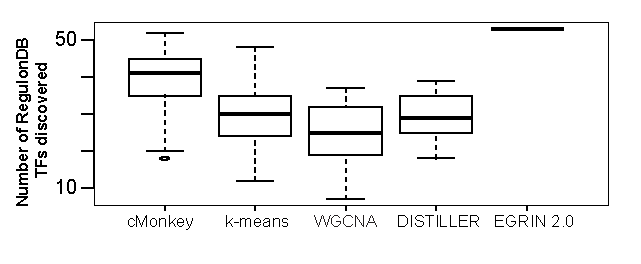
\includegraphics[width=0.6\linewidth]{figures/ensemble_comparison_regDB.pdf}
\caption[Number of TFs in \rdb~ re-discovered by various
    regulatory module detection methods.]  {{\bf Number of TFs in
    \rdb~ re-discovered by various regulatory module detection
    methods.} Comparison of \egrine~ (solid line, far right) to
  individual \cm\ runs, as well as multiple runs of $k$-means,
  \tmsamp{WGCNA}, and \tmsamp{DISTILLER} on subsets of the expression
  data. Evaluation made with respect to re-discovery of binding sites
  for 88 TFs with $\geq 3$ unique sites in \rdb~ based on genome-wide
  binding site locations (FDR $\leq 0.05$).}
\label{fig:ensemble_comparison_regDB}
\end{figure}

\subsection{Convergence and stability of the inferred network}

To evaluate the stability of the inferred \egrine\ network, we
quantified how the model changes as individual \cm\ runs are excluded
from the ensemble. Since the sub-bagging, as performed for
the \egrine\ model inference, %%(like cross-validation) is intended to
reduce model over-fitting, we used this evaluation understand whether
the model is over-fit to particular experiments in the data set. For
this task, we computed the number of individual EGRIN runs required to
converge on a consistent gene-gene co-occurrence network (see Section
\ref{section:gBg}). We computed gene-gene co-occurrence networks based upon randomly selected subsets of the 106 available \eco\ \cm\ runs, and varied the percentage selected between
1\%-99\% of the 106 runs. 5 replicate samples were computed for
each. To compare the networks, we computed the Pearson correlation
between the two matrices (sub-sampled gene-gene co-occurrence versus
the final \egrine\ gene-gene co-occurrence network). Note that since
the gene-gene co-occurrence network is a weighted adjacency matrix,
the correlation reflects the weighted discovery rate for every pair of
genes (rather than simple presence/absence). In
Figure \ref{fig:gBg_network_converge} we demonstrate that the
underlying networks converge rapidly to the final solution. By the
time $\sim 50$\% of the runs have been included ($\sim 50$ runs), the
inferred network is nearly identical to the final network ($\sim 100$
runs; cor $> 0.9$). The backbone extracted network takes a slightly
longer time to converge, likely because it requires more observations
of gene-gene pairs to retain them in the final network. Since corem
detection is deterministic and strictly based on the underlying
gene-gene co-occurrence matrix, this convergence means that the
inferred corems would be nearly identical even if up to half of the
runs were excluded.

\begin{figure}[h!]
\centering
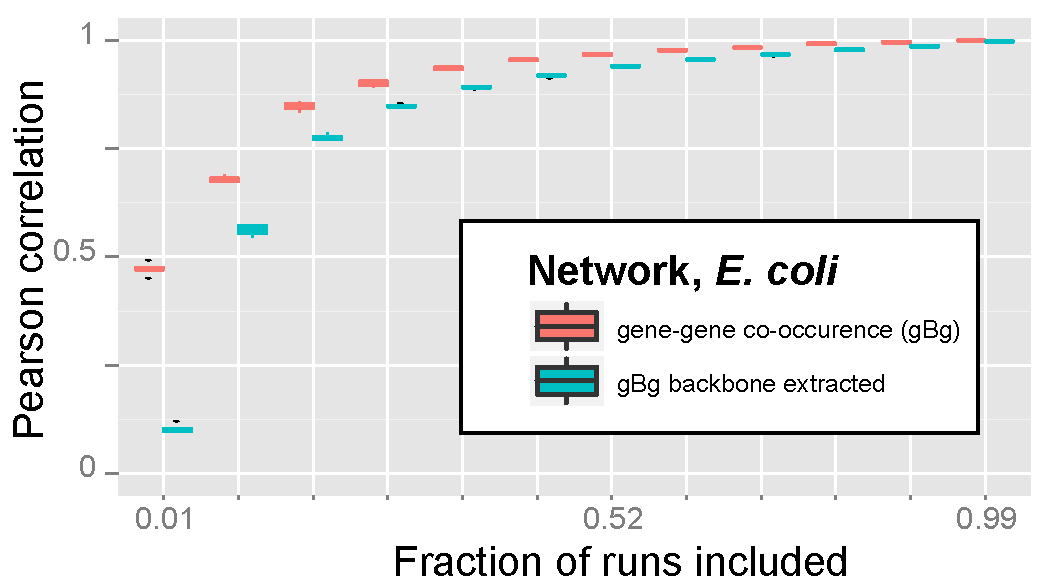
\includegraphics[width=0.75\linewidth]{figures/gBg_network_converge.pdf}
\caption[Convergence of \egrine\ gene co-occurrence networks.]  {
{\bf Convergence of \egrine\ co-occurrence networks.} The
co-regulation of genes predicted by the \eco\ \egrine\ model converges
rapidly to a stable network. Shown is the similarity of the gene-gene
co-occurrence matrix (and the backbone extraction of this matrix) to
the final \egrine\ \eco\ network, computed when varying fractions of
the \cm\ runs were excluded (Pearson correlation vs. the complete
model). Each point contains a box plot representing 5 replicate
sub-samples.}
\label{fig:gBg_network_converge}
\end{figure}

\subsection{Discovery of corems in an independent data set}

To determine whether \egrine\ model predictions are over-fit to
the \tmsamp{DISTILLER} expression compendium (or are the result of
biases in that data set), we tested whether support for corems existed
in an independent {\it E. coli} expression data set. Such evidence
would suggest that corems are \textit{bona fide} gene regulatory
modules that can be re-discovered in independent data, and that their
degree of condition-specificity is not biased due to normalization
differences in any given data set. For this test, we used
the \tmsamp{DREAM5} gene expression compendium. As described above
(Section \ref{section:dream5_data_compendium}), this data set is
comprised of different conditions, array platforms, and, most
important, was normalized by different methods, than
the \tmsamp{DISTILLER} data set used for model training. We determined
the condition-specific activity of corems in the \tmsamp{DREAM5} data
set using the methods described in Section \ref{section:rsd}. If a
corem was significantly co-expressed ($p$-value $\leq$ 0.05) in at
least one condition, we classified it `supported'. To our surprise, we
not only discovered support for $\sim 99$\% of the predicted corems,
we also discovered that their conditionality was very similar across
both data sets -- \ie, corems discovered to be co-expressed in few
conditions in the \tmsamp{DISTILLER} data set are also co-expressed in
few conditions in the \tmsamp{DREAM5} data set (same for corems
regulated in many conditions), and similarly for corems co-expressed
in a large number of conditions (Figure~\ref{fig:corem_conds_distiller_dream5}).
%% shows the number of conditions in which a corem is co-expressed across both data sets. 
Even after we removed the intrinsic relationship between the number of
genes in a corem and the number of conditions in which it is
co-expressed, we still observed a significant partial correlation of
0.49 ($p$-value $< 10^{-6}$) between the number of conditions in
corems as defined from the two data sets. 
%% The corems described in the main text({\color{red}ec512157}, {\color{blue}ec516034}, {\color{green}ec516031}) are indicated by their respective colors.

\begin{figure}[h!]
\centering
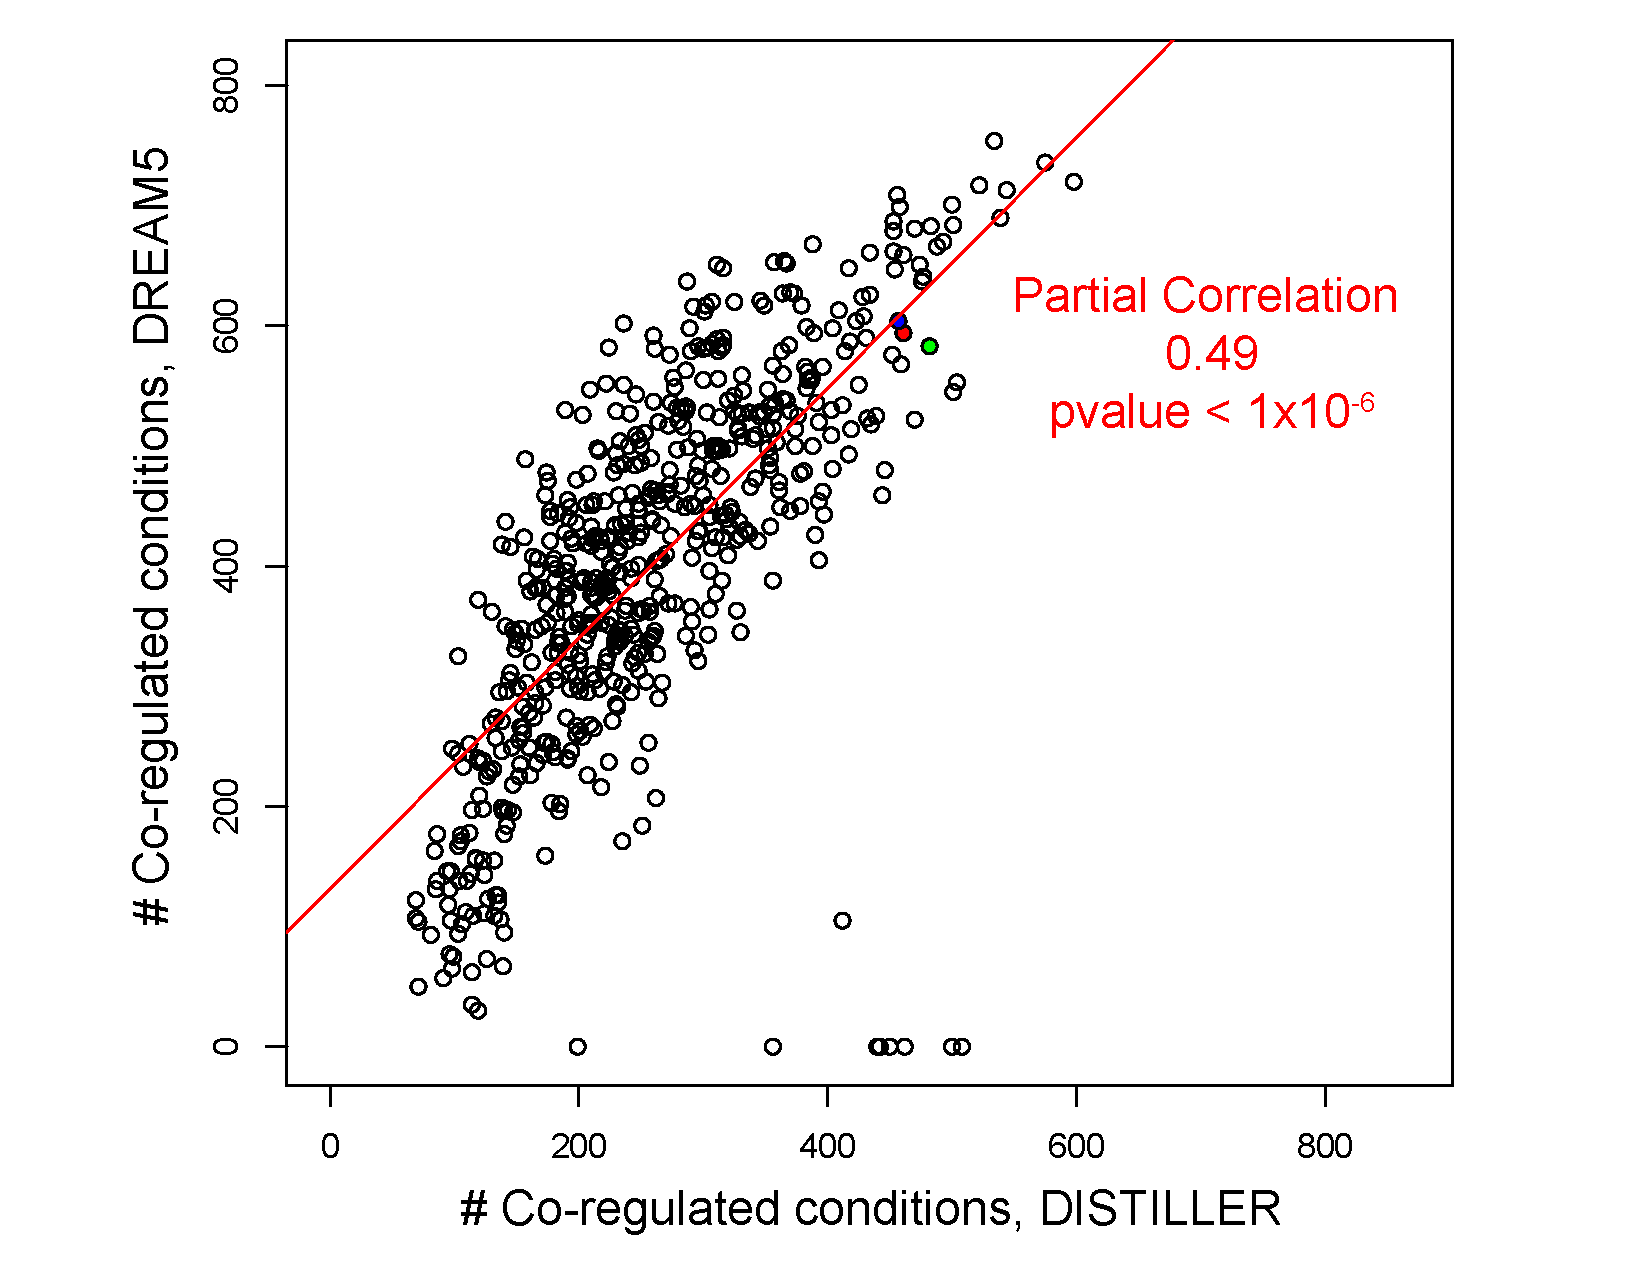
\includegraphics[width=0.6\linewidth]{figures/corem_conds_distiller_dream5.pdf}
\caption[Reproducibility of corems across data sets]{
\textbf{Reproducibility of corems across data sets.} 
Number of co-expressed conditions for corems in the \tmsamp{DISTILLER}
and \tmsamp{DREAM5} expression compendia. Conditions were selected as
in Section~\ref{section:rsd}. Significant partial correlation of 0.49
is observed after removing the affect of gene set size (log) on
the number of conditions co-expressed ($p$-value $< 10^{-6}$). The
three corems detailed in the main manuscript are identified with their
respective colors ({\color{red}ec512157}, {\color{blue}ec516034},
{\color{green}ec516031})}
\label{fig:corem_conds_distiller_dream5}
\end{figure}

